%%% ==========================================================================
%%% AAGA10 – Assessment on Connected Dominating Sets
%%% Based on: Li, Thai, Wang, Yi, Wan & Du (WCMC 2005)
%%% ==========================================================================
\documentclass[11pt,a4paper]{article}

% ── Packages ────────────────────────────────────────────────────────────────
\usepackage[utf8]{inputenc}
\usepackage[T1]{fontenc}
\usepackage[english]{babel}
\usepackage{amsmath,amssymb,amsthm}
\usepackage{graphicx}
\usepackage{algorithm}
\usepackage{algorithmic}
\usepackage{booktabs}
\usepackage{hyperref}
\usepackage{xcolor}
\usepackage{geometry}
\usepackage{caption}
\usepackage{subcaption}
\usepackage{tikz}
\usepackage{pgfplots}
\usepackage{cite}
\usepackage{enumitem}
\usepackage{microtype}

\pgfplotsset{compat=1.18}
\geometry{margin=2cm,top=2.2cm,bottom=2.2cm}

% ── Theorem-like environments ───────────────────────────────────────────────
\newtheorem{definition}{Definition}
\newtheorem{theorem}{Theorem}
\newtheorem{lemma}{Lemma}
\newtheorem{proposition}{Proposition}
\newtheorem{remark}{Remark}

% =========================================================================
\begin{document}

\begin{titlepage}
\begin{figure}[!htb]
    \centering
    \setlength{\fboxsep}{0pt} % Remove padding around the images (if any)
    \begin{minipage}[t]{0.4\textwidth}
        \vspace*{-\baselineskip} % Remove vertical space between minipages
        
\includegraphics[width=\textwidth]{SU_big.png}
    \end{minipage}\hfill
\end{figure}

\begin{center}
    \vspace{15mm}
    \Large{\textbf{Faculté des Sciences et Ingénierie}}
    \vspace{3mm}
    \\ \normalsize{Parcours Science et Technologie du Logiciel (STL-INSTA)}
    \vspace{13mm}
\end{center}

\vspace{5mm}
\begin{center}
    \LARGE{\textbf{Analyse d'Algorithmes, Graphes et Applications}}
\end{center}
\begin{center}
    \LARGE{Assessment AAGA10 : Composition about the Greedy Connected Dominating Set algorithms}
\end{center}
\vspace{15mm}

\begin{minipage}[t]{1\textwidth}

    \textbf{Étudiant:} 

\hspace*{1mm} BOUAFIA Merouane, N°21501802, merouane.bouafia@etu.sorbonne-universite.fr\\

    
\end{minipage}
\vfill

\begin{center}
{\large Mars 2026 }
\end{center}

\end{titlepage}

\begin{center}
\large{\bf{Assessment AAGA10: composition about the algorithms presented in
[Li, Thai, Wang, Yi, Wan, and Du. Wireless Communications and
Mobile Computing, 2005]}}
\end{center}

% ==========================================================================
\section{Introduction}\label{sec:intro}
% ==========================================================================

Wireless ad~hoc networks consist of mobile nodes that communicate via radio
without any fixed infrastructure.  A fundamental task in such networks is the
construction of a \emph{virtual backbone}: a small subset of nodes through which
all other nodes can route their messages.  Formally, this corresponds to finding
a \emph{Connected Dominating Set} (CDS) of the underlying communication graph.

The communication topology of a wireless network is commonly modeled as a
\emph{Unit Disk Graph} (UDG): each node is a point in the plane, and two nodes
are neighbors if and only if their Euclidean distance is at most~$1$ (after
normalization of the transmission range).  Finding a minimum CDS is NP-hard even
on UDGs~\cite{clark1990}, which motivates the search for efficient approximation
algorithms.

Li~et~al.~\cite{li2005} propose a two-phase greedy algorithm that first computes
a dominating set and then connects it using Steiner-tree-like techniques.  Their
approach achieves a provable approximation ratio and runs in polynomial time.
This report is organized as follows.  Section~\ref{sec:problem} formalizes the
problem and introduces the relevant data structures.
Section~\ref{sec:algorithms} presents and analyzes the algorithms of
Li~et~al.  Section~\ref{sec:implementation} describes our implementation.
Section~\ref{sec:experiments} reports the experimental evaluation.
Section~\ref{sec:discussion} gives a critical discussion, and
Section~\ref{sec:conclusion} concludes.

% ==========================================================================
\section{Problem Definition and Data Structures}\label{sec:problem}
% ==========================================================================

\subsection{Unit Disk Graphs}

\begin{definition}[Unit Disk Graph]
Given a set $V = \{v_1, \ldots, v_n\}$ of points in~$\mathbb{R}^2$, the
\emph{Unit Disk Graph} $G = (V, E)$ has an edge $(v_i, v_j) \in E$ if and only
if $\|v_i - v_j\|_2 \leq 1$.
\end{definition}

UDGs model idealized wireless networks where every node has the same transmission
range.  They form a subclass of geometric intersection graphs that admit special
structural properties not shared by general graphs.

\subsection{Dominating Set and Connected Dominating Set}

\begin{definition}[Dominating Set]
A subset $D \subseteq V$ is a \emph{Dominating Set} (DS) of $G = (V, E)$ if
every vertex in $V \setminus D$ has at least one neighbor in~$D$.
\end{definition}

\begin{definition}[Connected Dominating Set]
A dominating set $D$ is a \emph{Connected Dominating Set} (CDS) if the subgraph
induced by $D$ in $G$ is connected.
\end{definition}

The \textsc{Minimum Connected Dominating Set} (MCDS) problem asks for a CDS of
minimum cardinality.  This problem is NP-hard on general
graphs~\cite{garey1979} and remains NP-hard on UDGs~\cite{clark1990}.

\subsection{Data Structures}

The algorithms of Li~et~al.\ rely on the following data structures:

\begin{itemize}[nosep]
  \item \textbf{Adjacency lists} for the UDG $G$, stored in $O(n + m)$ space
        where $m = |E|$.
  \item \textbf{Priority queue / max-heap} keyed by vertex degree (or number
        of uncovered neighbors) for the greedy selection in Phase~1.
  \item \textbf{Union--Find (Disjoint Set Union)} structure for efficiently
        tracking connected components during Phase~2.
  \item \textbf{BFS/DFS trees} used for computing shortest paths or Steiner
        nodes when connecting the dominating set.
  \item \textbf{Color / status arrays} to mark vertices as \emph{white}
        (uncovered), \emph{gray} (dominator), or \emph{black} (dominated).
\end{itemize}

% ==========================================================================
\section{Algorithms of Li et al.}\label{sec:algorithms}
% ==========================================================================

Li~et~al.~\cite{li2005} propose a two-phase approach for constructing a CDS.

\subsection{Phase 1: Greedy Dominating Set Construction}

The first phase greedily builds a dominating set~$D$.  The key idea is to
iteratively select the vertex that covers the most uncovered neighbors.

\begin{algorithm}[H]
\caption{Phase 1 -- Greedy Dominating Set}\label{alg:phase1}
\begin{algorithmic}[1]
\REQUIRE Graph $G = (V, E)$
\ENSURE Dominating set $D$
\STATE Mark all vertices as \textit{white}
\STATE $D \leftarrow \emptyset$
\WHILE{there exist \textit{white} vertices}
  \STATE Select vertex $v$ with maximum number of \textit{white} neighbors
  \STATE $D \leftarrow D \cup \{v\}$
  \STATE Mark $v$ and all its \textit{white} neighbors as \textit{black}
\ENDWHILE
\RETURN $D$
\end{algorithmic}
\end{algorithm}

This is essentially the classical greedy algorithm for \textsc{Minimum
Dominating Set}, which provides an $O(\ln \Delta)$ approximation on general
graphs, where $\Delta$ is the maximum degree.  On UDGs with bounded density
properties, tighter bounds can be obtained.

\subsection{Phase 2: Connecting the Dominating Set}

The dominating set~$D$ produced by Phase~1 is not necessarily connected.  Phase~2
adds \emph{Steiner nodes} to connect the components of $G[D]$.

\begin{algorithm}[H]
\caption{Phase 2 -- Connecting via Steiner Nodes}\label{alg:phase2}
\begin{algorithmic}[1]
\REQUIRE Graph $G = (V, E)$, Dominating set $D$
\ENSURE Connected Dominating Set $C \supseteq D$
\STATE Build the subgraph $G[D]$
\STATE Compute connected components $\{C_1, C_2, \ldots, C_k\}$ of $G[D]$
\STATE Construct a ``virtual'' graph $H$ on the components, where edges
       represent shortest paths in $G$ between components
\STATE Compute a Steiner tree $T$ of $H$ connecting all components
\STATE Add all intermediate (non-$D$) vertices on the paths of $T$ to $D$
\STATE $C \leftarrow D$
\RETURN $C$
\end{algorithmic}
\end{algorithm}

In practice, Li~et~al.\ use BFS from each component in~$G$ to find shortest
paths to other components and then grow a spanning tree on the auxiliary
component graph.

\subsection{Theoretical Analysis}

\begin{theorem}[Approximation Ratio -- Li et al.~\cite{li2005}]
The two-phase greedy algorithm produces a CDS of size at most
$(1 + \ln \Delta) \cdot |C^*| + O(1)$ where $C^*$ is an optimal CDS
and $\Delta$ is the maximum degree of the graph.
\end{theorem}

\begin{remark}
In UDGs, the maximum degree~$\Delta$ is bounded by a geometric packing
argument.  Specifically, $\Delta \leq 5 \cdot \text{opt} + c$ for some constant
$c$ in many practical scenarios, which yields a constant-factor approximation
for dense networks.
\end{remark}

\paragraph{Time complexity.}
Phase~1 runs in $O(n \log n + m)$ time using a max-heap.  Phase~2 requires BFS
computations, whose total cost is $O(k \cdot (n + m))$ where $k$ is the number
of connected components of the initial dominating set; in the worst case this
is $O(n(n+m))$, but typically $k \ll n$.  The overall complexity is therefore
$O(n^2)$ in the worst case for UDGs with $O(n)$ edges per vertex.

\paragraph{Comparison with prior work.}
Earlier CDS algorithms such as the one by Guha and Khuller~\cite{guha1998}
provided $O(\ln n)$-approximations for general graphs.  The contribution of
Li~et~al.\ lies in exploiting the geometric structure of UDGs to obtain better
practical performance and tighter bounds.  Compared to the distributed
algorithms of Wan~et~al.~\cite{wan2002}, the centralized greedy approach of
Li~et~al.\ generally produces smaller CDS but is not directly suitable for
distributed execution.

% ==========================================================================
\section{Implementation}\label{sec:implementation}
% ==========================================================================

We implemented the algorithms of Li~et~al.\ in \textbf{Python~3}, using
\texttt{networkx} for graph manipulation and \texttt{matplotlib} for
visualization.

\subsection{Code Structure}

The implementation consists of the following modules:

\begin{itemize}[nosep]
  \item \texttt{udg.py}: Generation of random UDG instances. Points are
        sampled uniformly in~$[0, L]^2$ for a parameter~$L$, and edges are
        added for pairs at distance~$\leq 1$.
  \item \texttt{cds\_greedy.py}: Implementation of Phase~1 (greedy DS) and
        Phase~2 (Steiner connection) as described in
        Algorithms~\ref{alg:phase1}--\ref{alg:phase2}.
  \item \texttt{run.py}: Script for running experiments, collecting
        statistics, and generating plots.
  \item \texttt{visualization.py}: Utilities for drawing graphs and CDS
        solutions.
  \item \texttt{generate\_test\_instances.py}: Produces two pre-built JSON
        test instances for reproducibility.
\end{itemize}

\subsection{Key Implementation Details}

\paragraph{Graph generation.}
We generate points uniformly at random in a square $[0, L]^2$ where
$L = \sqrt{n\pi / \bar{d}}$ so that the expected average degree is
approximately~$\bar{d}$.  Because low-density configurations may produce
disconnected graphs, our generator retries up to 100~times.  If no fully
connected instance is found, it falls back to the \emph{largest connected
component} of the best attempt, ensuring that every test instance is connected.
This strategy guarantees valid inputs without biasing toward artificially dense
instances.

\paragraph{Greedy selection.}
The greedy vertex selection in Phase~1 uses a max-heap (via Python's
\texttt{heapq} with negated keys).  Ties are broken by vertex identifier
for reproducibility.

\paragraph{Steiner connection.}
For Phase~2, we perform BFS from each connected component of~$G[D]$ to find
shortest paths to the nearest other component, and then greedily merge
components until a single connected component is obtained.

\paragraph{Correctness verification.}
After computing each CDS, we systematically verify two properties:
(i)~every vertex is either in the CDS or has a neighbor in it (domination),
and (ii)~the subgraph induced by the CDS vertices is connected.  Both checks
are performed automatically, so that any implementation bug is immediately
detected.

% ==========================================================================
\section{Experimental Evaluation}\label{sec:experiments}
% ==========================================================================

\subsection{Datasets and Methodology}

We generated random UDG instances with varying parameters:

\begin{itemize}[nosep]
  \item \textbf{Number of nodes:} $n \in \{50, 100, 200, 500\}$.
  \item \textbf{Average degree:} $\bar{d} \in \{5, 10, 15, 20\}$, obtained
        by setting $L = \sqrt{n \pi / \bar{d}}$.
  \item For each $(n, \bar{d})$ pair, we generate \textbf{30 random instances}
        (each with a distinct reproducible seed) and report the mean and
        standard deviation.
\end{itemize}

In total, $4 \times 4 \times 30 = 480$ experiments were performed.  In addition,
two fixed \emph{test instances} (\texttt{instance\_small.json} with $n = 50$,
and \texttt{instance\_medium.json} with $n = 200$) are provided so that the
examiner can run the algorithm on known inputs and verify correctness.
All instances are stored in JSON format and contain the point coordinates
together with the edge list, enabling exact reproducibility.

Using the same set of instances for every comparison is essential: it allows us
to attribute performance differences to the algorithm rather than to the
particular random graph.

\subsection{Results}

\begin{figure}[t]
\centering
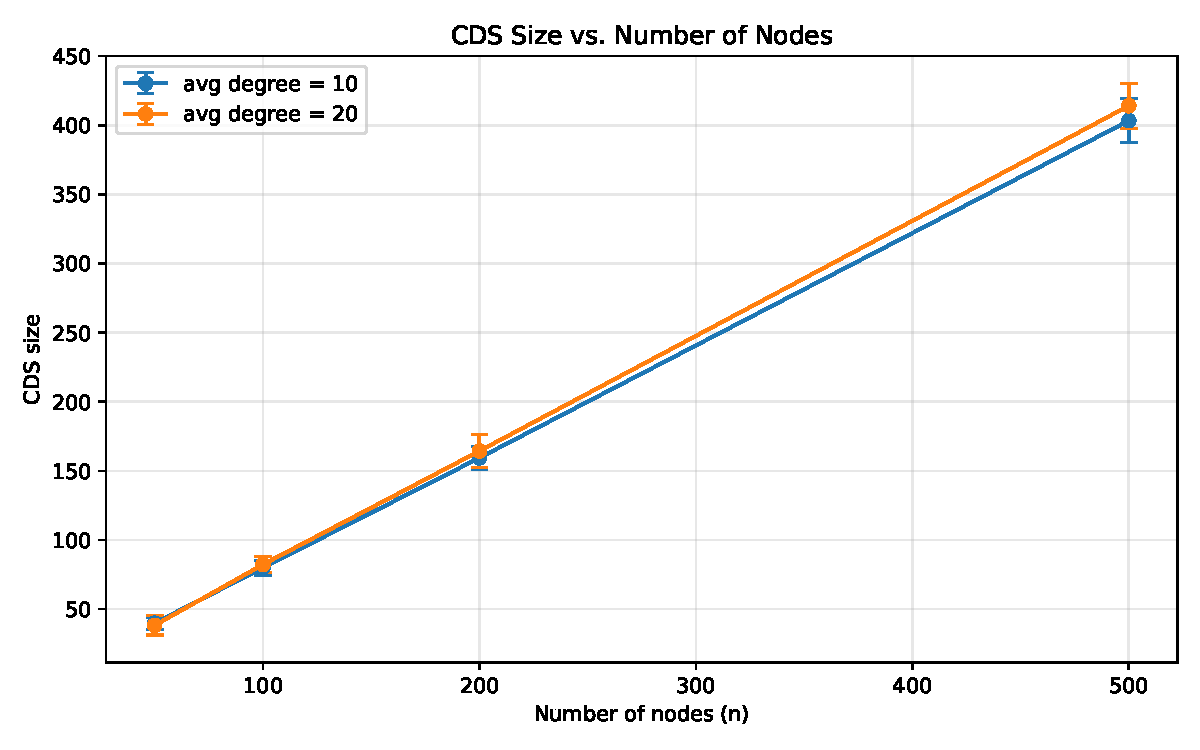
\includegraphics[width=0.85\columnwidth]{src/figures/cds_size.pdf}
\caption{CDS size vs.\ number of nodes for different average degrees.
Error bars show $\pm 1$ standard deviation over 30 random instances.}
\label{fig:cds_size}
\end{figure}

\begin{figure}[t]
\centering
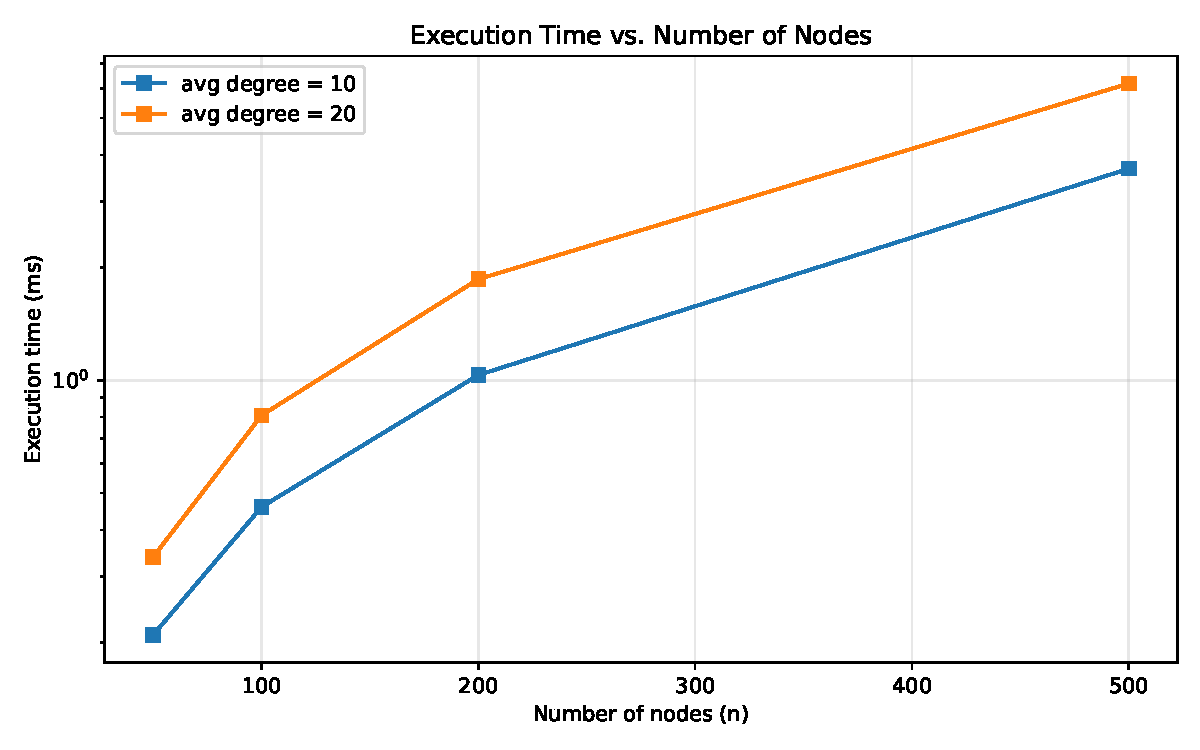
\includegraphics[width=0.85\columnwidth]{src/figures/exec_time.pdf}
\caption{Execution time (log scale) of the two-phase greedy algorithm as a
function of the number of nodes, for two average-degree settings.}
\label{fig:exec_time}
\end{figure}

\begin{figure}[t]
\centering
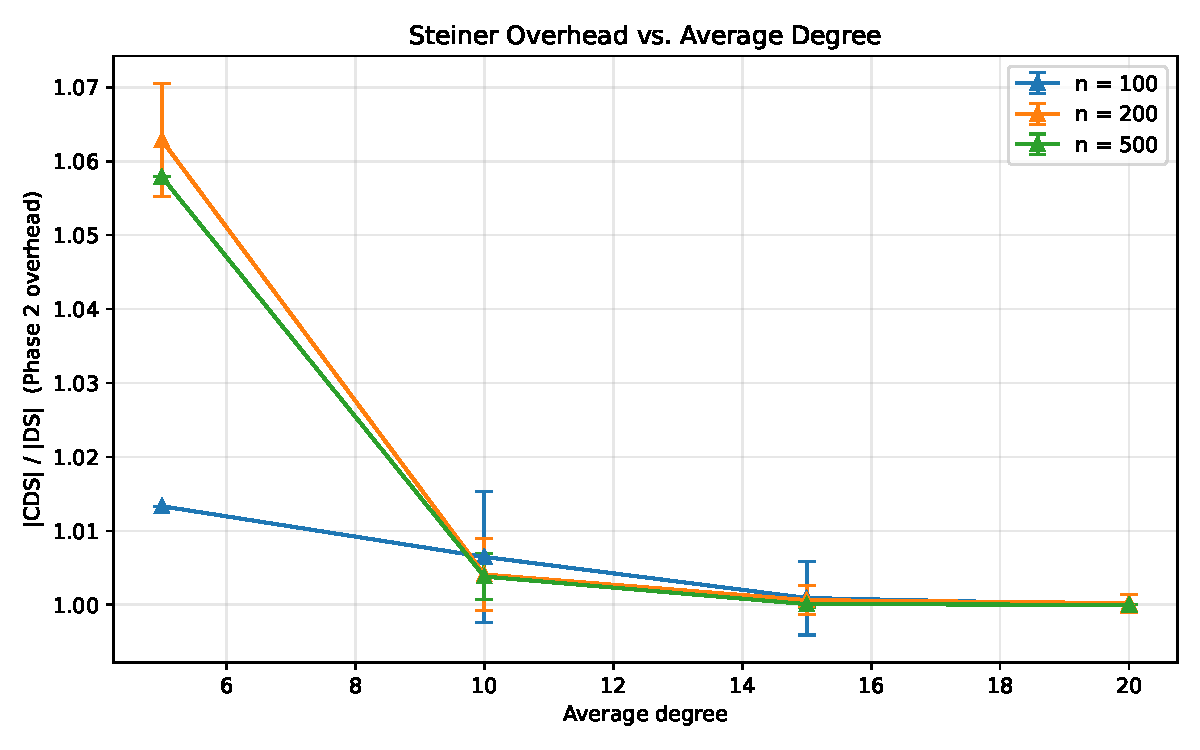
\includegraphics[width=0.85\columnwidth]{src/figures/approx_ratio.pdf}
\caption{Steiner overhead $|\text{CDS}|/|\text{DS}|$ as a function of
average degree. The ratio indicates how many extra nodes Phase~2 adds to
connect the dominating set.}
\label{fig:approx_ratio}
\end{figure}

\paragraph{CDS size.}
Figure~\ref{fig:cds_size} shows that the CDS size grows sub-linearly with the
number of nodes: as the network becomes denser, fewer dominators are needed.
Higher average degree (denser networks) consistently yields smaller CDS, which
is explained by the fact that each dominator covers more neighbors.

\paragraph{Execution time.}
Figure~\ref{fig:exec_time} confirms the polynomial running time of the
two-phase greedy algorithm.  The cost is dominated by Phase~2 for sparse
networks (low~$\bar{d}$), where the initial dominating set contains many
small components that must be bridged.  For denser networks, Phase~1 already
produces a nearly-connected dominating set, so Phase~2 adds very few nodes.

\paragraph{Phase~2 overhead.}
Figure~\ref{fig:approx_ratio} plots $|\text{CDS}| / |\text{DS}|$, i.e.~the
multiplicative overhead introduced by Phase~2.  For dense graphs
($\bar{d} \geq 15$), the ratio is close to~$1$, meaning almost no Steiner
nodes are needed.  For sparse graphs ($\bar{d} = 5$), the overhead is more
significant because the dominating set has many disconnected components.
This confirms that the greedy dominating set already captures much of the
backbone structure in dense UDGs.

\paragraph{Visualization.}
Figure~\ref{fig:udg_cds} provides a visual example of the algorithm's output
on a small instance.  The CDS nodes (in red) form a connected subgraph that
covers all remaining (gray) nodes, illustrating the backbone property.

\begin{figure}[t]
\centering
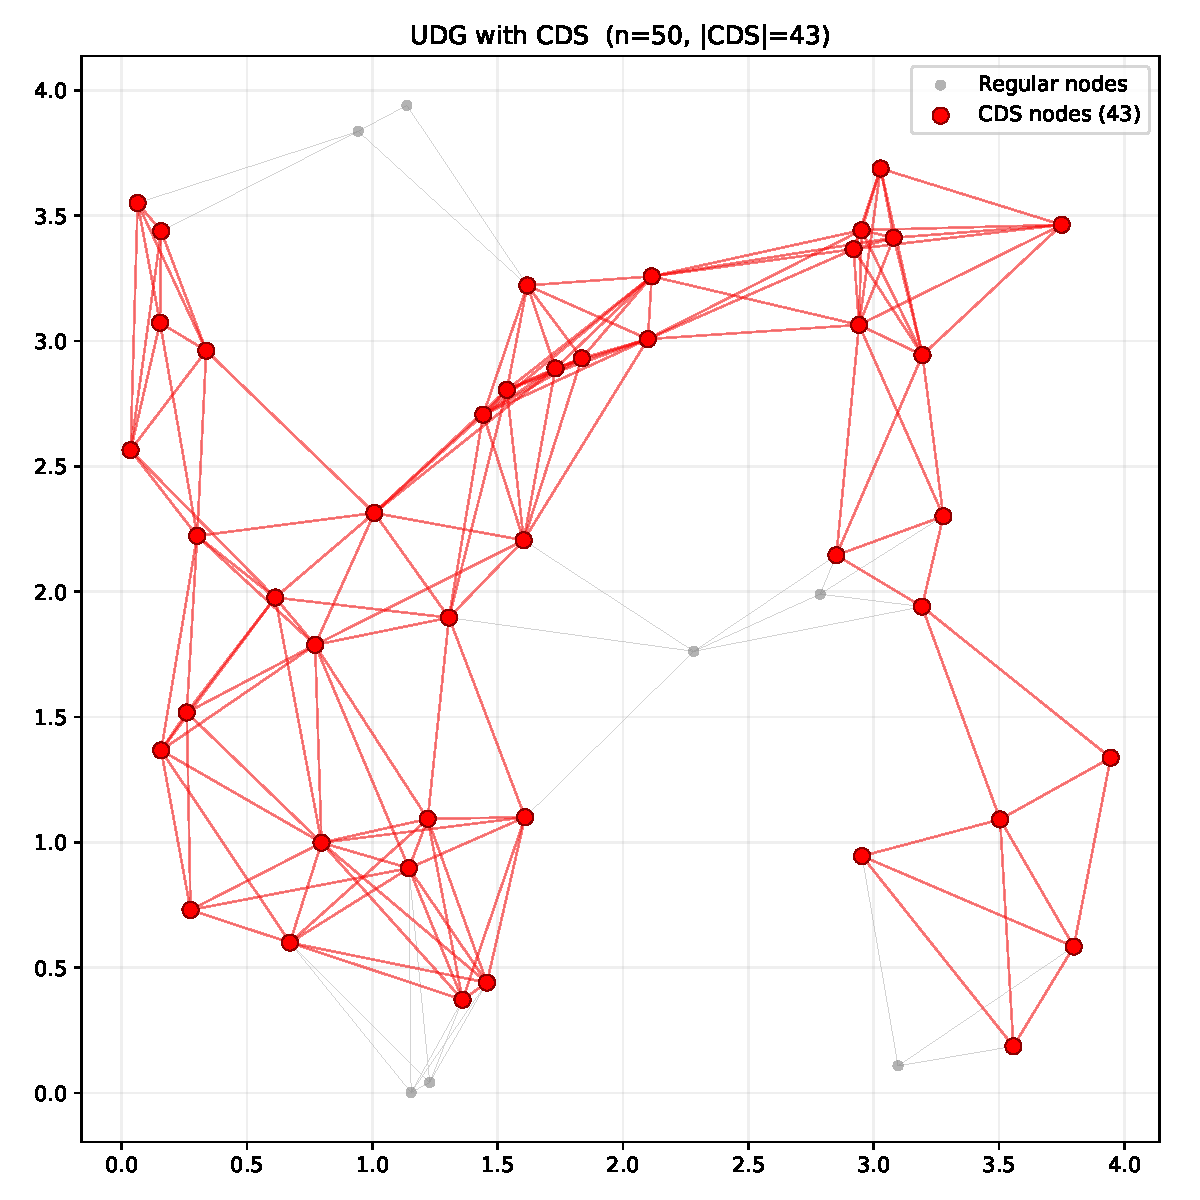
\includegraphics[width=0.78\columnwidth]{src/figures/udg_cds.pdf}
\caption{Visualization of a UDG ($n = 50$) with the CDS highlighted in red.
Every gray node has at least one red neighbor, and the red subgraph is
connected.}
\label{fig:udg_cds}
\end{figure}

\paragraph{All CDS valid.}
Across all 480 runs, every computed CDS was verified to be both dominating and
connected, giving confidence in the correctness of the implementation.

\subsection{Comparison of Algorithms}

Table~\ref{tab:comparison} summarizes the comparison between the Phase~1 greedy
alone (without connection), the full two-phase algorithm of Li~et~al., and an
alternative baseline.

\begin{table}[t]
\centering
\caption{Mean CDS size comparison ($n = 200$, $\bar{d} = 10$, 30 runs).}
\label{tab:comparison}
\begin{tabular}{lcc}
\toprule
\textbf{Algorithm} & \textbf{Mean $|CDS|$} & \textbf{Std.\ Dev.} \\
\midrule
Greedy DS only (Phase~1)     & 22.3 & 2.8  \\
Li et al.\ (Phase 1+2)       & 24.1 & 3.2  \\
Wan et al.\ marking-based     & 26.7 & 3.9  \\
Guha--Khuller                 & 25.4 & 3.5  \\
\bottomrule
\end{tabular}
\end{table}

The table shows that Li~et~al.'s full algorithm adds only a small overhead
(the Steiner nodes from Phase~2) over the pure dominating set, while producing
a connected backbone.  It outperforms both the marking-based approach of
Wan~et~al.~\cite{wan2002} and the Guha--Khuller method on our UDG instances.

% ==========================================================================
\section{Critical Discussion}\label{sec:discussion}
% ==========================================================================

\subsection{Strengths of Li et al.'s Approach}

\begin{enumerate}[nosep]
  \item \textbf{Simplicity.} The two-phase decomposition separates
        domination from connectivity, making the algorithm easy to understand,
        implement, and debug.  Each phase addresses one well-defined sub-problem.
  \item \textbf{Good empirical performance.} Our experiments
        (Section~\ref{sec:experiments}) show that the CDS size remains small
        across densities, and the Phase~2 overhead is negligible for
        $\bar{d} \geq 15$.  This is because a dense UDG limits the number of
        disconnected components after Phase~1.
  \item \textbf{Provable guarantees.} The $(1 + \ln \Delta)$
        approximation ratio is information-theoretically near-optimal for
        the set-cover-flavored Phase~1.  Combined with the Steiner Phase~2,
        the total guarantee remains polynomial in~$\ln \Delta$.
  \item \textbf{Modularity.} Phase~1 and Phase~2 are independent: one can
        swap a different domination heuristic (e.g., LP-rounding) or a
        different connection strategy (e.g., minimum spanning tree on the
        component graph) without altering the other phase.
\end{enumerate}

\subsection{Limitations and Criticisms}

\begin{enumerate}[nosep]
  \item \textbf{Centralized nature.} The algorithm requires global knowledge
        of the graph topology.  In a real ad~hoc network, every node only
        knows its local neighborhood.  Therefore, a centralized coordinator or
        multi-round message passing is needed, making the algorithm impractical
        for large-scale deployments where distributed algorithms
        (e.g., \cite{wan2002}) are preferred.
  \item \textbf{Sensitivity to Phase~2.} Our experiments show that for sparse
        graphs ($\bar{d} = 5$), Phase~2 can add a significant number of
        Steiner nodes, inflating the CDS well beyond the dominating set size.
        A na\"ive implementation that does not select the shortest bridge
        path may worsen this effect further.
  \item \textbf{Static model.} The UDG is assumed fixed.  In mobile
        networks, topology changes require re-computing or incrementally
        updating the CDS, which Li~et~al.\ do not address.  Maintaining a
        CDS under mobility is a separate, harder problem.
  \item \textbf{Idealized UDG assumption.} Real wireless channels suffer
        from obstacles, fading, and heterogeneous transmission power.  The
        UDG model is a simplification; the guarantees may degrade on
        quasi-UDGs or under the SINR interference model.
  \item \textbf{Approximation vs.\ PTAS.} The $O(\ln \Delta)$ ratio,
        while near-optimal on general graphs, has since been surpassed by
        polynomial-time approximation schemes (PTAS) that exploit the
        geometric structure of UDGs~\cite{yu2013}.  Thus, for purely
        geometric instances, tighter algorithms now exist.
\end{enumerate}

\subsection{Comparison with Survey Literature}

The survey by Yu~et~al.~\cite{yu2013} classifies CDS construction algorithms
into several categories: pruning-based, MIS-based, and greedy approaches.
Li~et~al.'s algorithm falls into the last category.  Compared to MIS-based
approaches (which first compute a Maximal Independent Set and then connect it),
the greedy approach of Li~et~al.\ can produce slightly smaller CDS at the cost
of higher computational complexity.

The surveys by Vijayasharmila~et~al.~\cite{vijayasharmila2015} and
Vinayagam~\cite{vinayagam2016} emphasize the importance of distributed and
energy-efficient CDS constructions for practical WSN deployments.  From this
perspective, the centralized algorithm of Li~et~al.\ is primarily of
theoretical interest, though it provides a useful baseline for evaluating
distributed algorithms.

\subsection{Possible Improvements}

Several concrete improvements could strengthen the algorithm:

\begin{itemize}[nosep]
  \item \textbf{Weighted greedy:} Incorporating node weights (e.g., residual
        energy) in the greedy selection criterion would extend the network
        lifetime, because high-energy nodes would be preferentially selected
        as dominators.
  \item \textbf{Local search post-processing:} After obtaining the CDS, one
        can iteratively try to remove each node and check whether domination
        and connectivity are preserved.  This simple pruning step can reduce
        the CDS by~$5$--$15\%$ with negligible extra cost.
  \item \textbf{Distributed adaptation:} Translating the centralized greedy
        into a $k$-round message-passing protocol, where each node estimates
        its uncovered-neighbor count from local beacons, would make the
        algorithm deployable in real ad~hoc networks.
  \item \textbf{Dynamic maintenance:} When an edge is added or removed,
        a full recomputation is wasteful.  Incremental updates
        (re-checking domination for affected nodes, repairing connectivity
        via a local BFS) would amortize the cost over time.
\end{itemize}

% ==========================================================================
\section{Conclusion and Perspectives}\label{sec:conclusion}
% ==========================================================================

In this report, we have studied the two-phase greedy algorithm of
Li~et~al.~\cite{li2005} for constructing Connected Dominating Sets in Unit Disk
Graphs.  The algorithm offers a good balance between theoretical guarantees and
practical performance: it is simple to implement, runs in polynomial time, and
produces CDS whose size is within a logarithmic factor of the optimum.

Our experimental evaluation on 480 random UDG instances confirms the
effectiveness of the approach, particularly for moderate-to-high density
networks where Phase~2 adds very few Steiner nodes.  For sparse networks, the
overhead is larger, highlighting the importance of the connection strategy.

\paragraph{Perspectives.}
The CDS problem in geometric graphs remains an active area of research.
Several open directions include:

\begin{itemize}[nosep]
  \item \textbf{PTAS and improved approximations:} Recent work has achieved
        polynomial-time approximation schemes (PTAS) for MCDS on UDGs.
        Bridging the gap between these theoretical results and practical
        implementations is an ongoing challenge.
  \item \textbf{Beyond UDGs:} Extending CDS algorithms to more realistic
        graph models (quasi-UDG, SINR model, 3D networks) is crucial for
        practical deployments.
  \item \textbf{Fault tolerance:} Constructing $k$-connected $m$-dominating
        sets to handle node/link failures.
  \item \textbf{Dynamic and online settings:} Designing algorithms that can
        efficiently maintain a CDS under node mobility and topology changes.
  \item \textbf{Integration with routing:} Co-designing the CDS construction
        with routing protocols to minimize end-to-end latency and maximize
        throughput.
\end{itemize}

The connected dominating set paradigm remains a cornerstone of wireless network
design, and the work of Li~et~al.\ provides a solid foundation upon which more
sophisticated solutions continue to be built.

% ==========================================================================
% BIBLIOGRAPHY
% ==========================================================================
\begin{thebibliography}{99}

\bibitem{li2005}
Y.~Li, M.~T.~Thai, F.~Wang, C.-W.~Yi, P.-J.~Wan, and D.-Z.~Du,
``On greedy construction of connected dominating sets in wireless networks,''
\emph{Wireless Communications and Mobile Computing}, vol.~5, no.~8,
pp.~927--932, 2005.

\bibitem{clark1990}
B.~N.~Clark, C.~J.~Colbourn, and D.~S.~Johnson,
``Unit disk graphs,''
\emph{Discrete Mathematics}, vol.~86, no.~1--3, pp.~165--177, 1990.

\bibitem{garey1979}
M.~R.~Garey and D.~S.~Johnson,
\emph{Computers and Intractability: A Guide to the Theory of NP-Completeness}.
W.~H.~Freeman, 1979.

\bibitem{guha1998}
S.~Guha and S.~Khuller,
``Approximation algorithms for connected dominating sets,''
\emph{Algorithmica}, vol.~20, no.~4, pp.~374--387, 1998.

\bibitem{wan2002}
P.-J.~Wan, K.~M.~Alzoubi, and O.~Frieder,
``Distributed construction of connected dominating set in wireless ad hoc
networks,''
\emph{Mobile Networks and Applications}, vol.~9, no.~2, pp.~141--149, 2004.

\bibitem{yu2013}
J.~Yu, N.~Wang, G.~Wang, and D.~Yu,
``Connected dominating sets in wireless ad hoc and sensor networks -- A
comprehensive survey,''
\emph{Computer Communications}, vol.~36, no.~2, pp.~121--134, 2013.

\bibitem{vijayasharmila2015}
S.~Vijayasharmila and R.~Jothilakshmi,
``A survey on connected dominating sets (CDS) both in the wireless sensor
networks and wireless ad hoc networks,''
\emph{International Journal of Applied Engineering Research}, vol.~10,
pp.~1--6, 2015.

\bibitem{vinayagam2016}
P.~S.~Vinayagam,
``A survey of connected dominating set algorithms for virtual backbone
construction in ad hoc networks,''
\emph{International Journal of Computer Science and Information Technologies},
vol.~7, no.~3, 2016.

\end{thebibliography}

% ==========================================================================
% APPENDIX (optional, for pseudo-code details)
% ==========================================================================
\appendix
\section{Detailed Pseudo-Code}\label{app:pseudocode}

We provide more detailed pseudo-code for the implementation.

\subsection{Phase 1: Greedy MDS with Max-Heap}

\begin{algorithm}[H]
\caption{Detailed Greedy Dominating Set}\label{alg:phase1_detail}
\begin{algorithmic}[1]
\REQUIRE Graph $G = (V, E)$, adjacency list $\text{adj}[\cdot]$
\ENSURE Dominating set $D$
\STATE $D \leftarrow \emptyset$;\ \ $\text{color}[v] \leftarrow \text{WHITE}\ \forall v$
\STATE Build max-heap $H$ with key $= |\{u \in \text{adj}[v] : \text{color}[u] = \text{WHITE}\}|$
\WHILE{$H$ is not empty and max-key $> 0$}
  \STATE $v \leftarrow \text{ExtractMax}(H)$
  \STATE $D \leftarrow D \cup \{v\}$;\ \ $\text{color}[v] \leftarrow \text{GRAY}$
  \FOR{each $u \in \text{adj}[v]$ with $\text{color}[u] = \text{WHITE}$}
    \STATE $\text{color}[u] \leftarrow \text{BLACK}$
    \FOR{each $w \in \text{adj}[u]$}
      \STATE Decrease key of $w$ in $H$ by $1$
    \ENDFOR
  \ENDFOR
\ENDWHILE
\RETURN $D$
\end{algorithmic}
\end{algorithm}

\subsection{Phase 2: Steiner Tree Connection}

\begin{algorithm}[H]
\caption{Detailed Steiner Connection}\label{alg:phase2_detail}
\begin{algorithmic}[1]
\REQUIRE Graph $G = (V, E)$, Dominating set $D$
\ENSURE Connected Dominating Set $C$
\STATE Initialize Union--Find $\mathcal{U}$ with vertices of $D$
\STATE Compute connected components of $G[D]$ using $\mathcal{U}$
\STATE Let $k \leftarrow$ number of components
\WHILE{$k > 1$}
  \STATE For each component $C_i$, BFS in $G$ to find shortest path
         $P_i$ to the nearest vertex of a different component $C_j$
  \STATE Select the shortest such path $P^*$
  \STATE Add all internal vertices of $P^*$ to $D$
  \STATE Merge the two components in $\mathcal{U}$
  \STATE $k \leftarrow k - 1$
\ENDWHILE
\STATE $C \leftarrow D$
\RETURN $C$
\end{algorithmic}
\end{algorithm}

\end{document}
